Como el codigo fue creciendo de a poco, notamos que, de equivocarnos en una seccion que era utilizada por otras, implicaba tocar todos los documentos una y otra vez, para resolver el error. Para solucionar esto optamos por aislar de alguna forma las secciones con una capa intermedia, la cual guardaria toda la informacion necesaria para el sistema y la expondria a cada seccion, solo el tipo de datos necesario. Por ejemplo, como tenemos 3 tipos de direcciones:fisica, virtual y de pantalla, centramos todas las conversiones entre estas tres en un modulo que llamamos "Context Manager" y cada seccion solo recibe el tipo de direccion que requiere, sin tener que incluir en el codigo las conversiones.\\

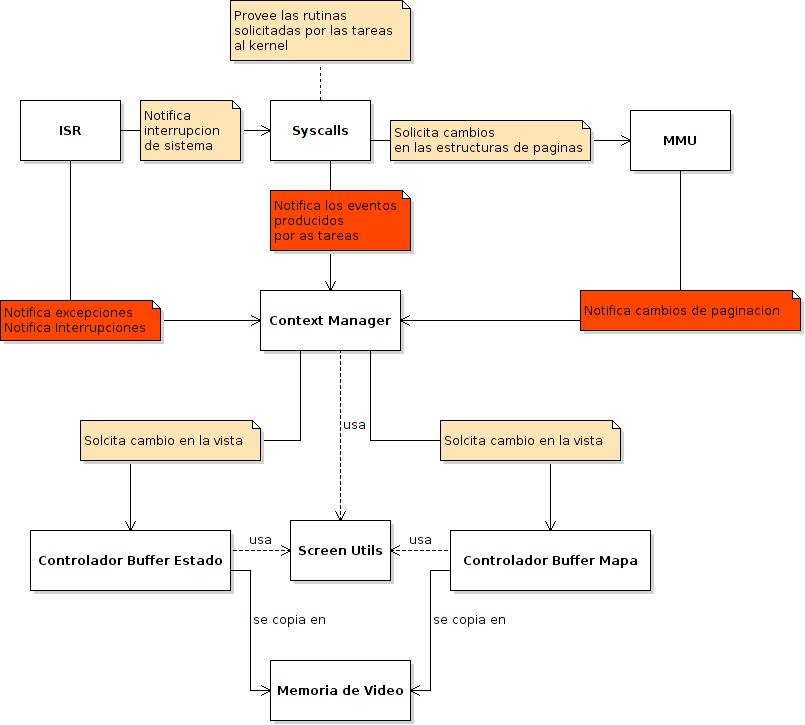
\includegraphics[scale=0.5]{diagramas/contextManager-relaciones.jpg}   
\\Context Manager y sus relaciones con las demas secciones. Imagen sin especificar las funciones internas\\

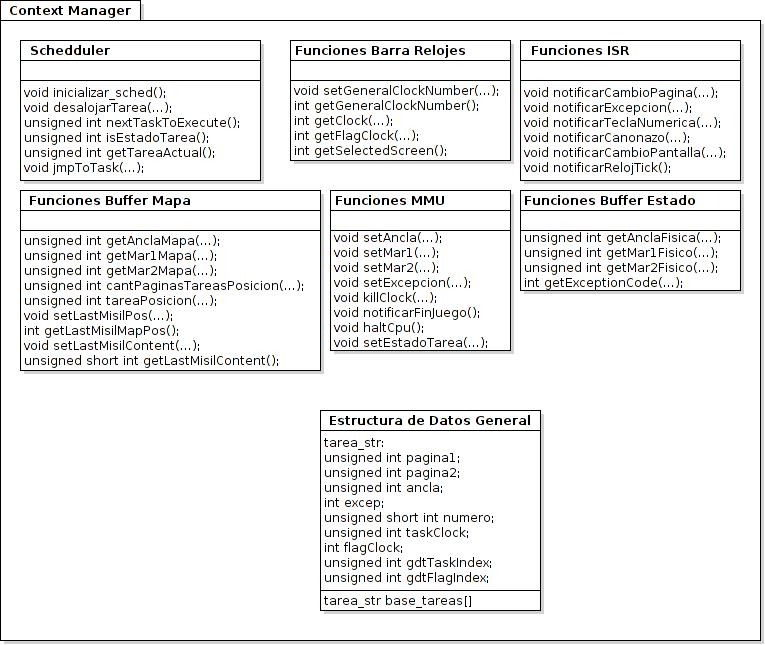
\includegraphics[scale=0.5]{diagramas/contextManager.jpg}   
\\Funciones y estructuras del Context Manager\\


Siendo de esta forma un paso intermedio entre las partes, la secuencia de accion de cada funcionalidad del juego pasa por el mismo. En las siguientes secciones se mostrara como las distintas funcionalidades utilizan esta estructura.
